\documentclass{standalone}
\usepackage{tikz}
\usetikzlibrary{arrows.meta}
\renewcommand{\familydefault}{\sfdefault} % Sans serif

\tikzset{
	partial ellipse/.style args={#1:#2:#3}{
		insert path={+ (#1:#3) arc (#1:#2:#3)}
	}
}

\begin{document}	
	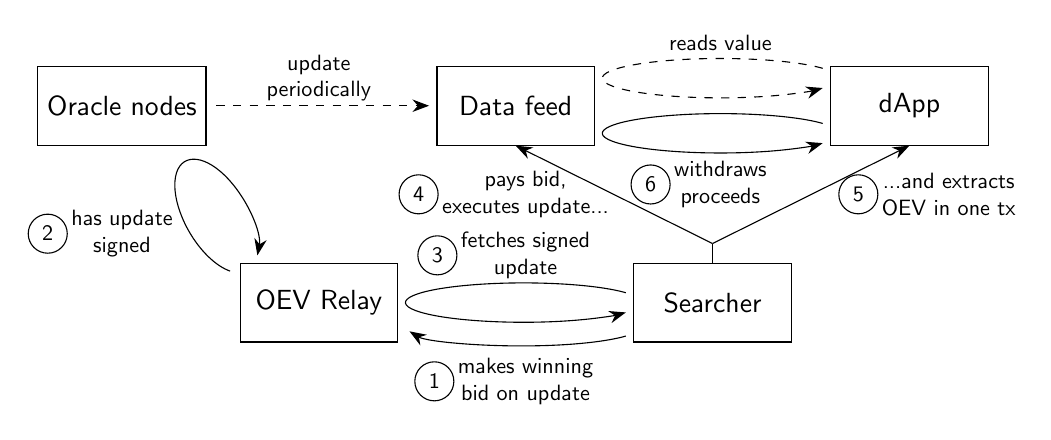
\begin{tikzpicture}
	\node[draw, minimum width=2cm,minimum height=1cm, align=center] at (0,0) (oracle-nodes) {Oracle nodes};
	\node[draw, minimum width=2cm,minimum height=1cm, align=center] at (5,0) (data-feed) {Data feed};
	\node[draw, minimum width=2cm,minimum height=1cm, align=center] at (10,0) (dapp) {dApp};
	\node[draw, minimum width=2cm,minimum height=1cm, align=center] at (2.5,-2.5) (oev-relay) {OEV Relay};
	\node[draw, minimum width=2cm,minimum height=1cm, align=center] at (7.5,-2.5) (searcher) {Searcher};
	
	\draw[{Stealth[scale=1.25]}-] (5.1,-2.8) [partial ellipse=-165:-30:1.5cm and 0.25cm];
	\node[align=center, scale=0.8] at (5.125, -3.5) (step-1-text) {makes winning\\bid on update};
	\node[draw, circle, align=center, scale=0.8] at ([shift=({-2mm,0})]step-1-text.west) (step-1) {1};
	
	\draw[{Stealth[scale=1.25]}-, rotate around={300:(1.2,-1.4)}] (1.2,-1.4) [partial ellipse=30:330:0.8cm and 0.4cm];
	\node[align=center, scale=0.8] at (0, -1.625) (step-2-text) {has update\\signed};
	\node[draw, circle, align=center, scale=0.8] at ([shift=({-2mm,0})]step-2-text.west) (step-2) {2};

	\draw[-{Stealth[scale=1.25]}] (5.1,-2.5) [partial ellipse=30:330:1.5cm and 0.25cm];
	\node[align=center, scale=0.8] at (5.125, -1.9) (step-3-text) {fetches signed\\update};
	\node[draw, circle, align=center, scale=0.8] at ([shift=({-2mm,0})]step-3-text.west) (step-3) {3};

	\draw (searcher.north) to (7.5,-1.75);
	\draw[-{Stealth[scale=1.25]}] (7.5,-1.75) to (data-feed.south);
	\node[align=center, scale=0.8] at (5.125, -1.125) (step-4-text) {pays bid,\\executes update...};
	\node[draw, circle, align=center, scale=0.8] at ([shift=({-2mm,0})]step-4-text.west) (step-4) {4};
	\draw[-{Stealth[scale=1.25]}] (7.5,-1.75) to (dapp.south);
	\node[align=center, scale=0.8] at (10.5, -1.125) (step-5-text) {...and extracts\\OEV in one tx};
	\node[draw, circle, align=center, scale=0.8] at ([shift=({-2mm,0})]step-5-text.west) (step-5) {5};
	
	\draw[-{Stealth[scale=1.25]}] (7.6,-0.35) [partial ellipse=30:330:1.5cm and 0.25cm];
	\node[align=center, scale=0.8] at (7.6, -1) (step-6-text) {withdraws\\proceeds};
	\node[draw, circle, align=center, scale=0.8] at ([shift=({-2mm,0})]step-6-text.west) (step-6) {6};
	
	\draw[-{Stealth[scale=1.25]}, dashed] (1.2,0) to (3.9,0);
	\node[align=center, scale=0.8] at (2.5, 0.35) {update\\periodically};
	
	\draw[-{Stealth[scale=1.25]}, dashed] (7.6,0.35) [partial ellipse=30:330:1.5cm and 0.25cm];
	\node[align=center, scale=0.8] at (7.6, 0.8) {reads value};
	\end{tikzpicture}
\end{document}